\subsection{Output System}
\schematicpage{4}{OutputAmp}

\subsubsection{Attenuator and Filter}
\subsubsection{Gain Stages and Termination}

\subsection{Input System}
\schematicpage{6}{InputFrontend}

The input system is used to transform the signals received from the device
under test into signals that can be read directly by the microcontroller.
First, the signals pass through a protection network; this is to protect
the following (expensive!) circuitry from damage by signals that are too
large. The signals then pass into a switch, allowing one of the two to be
selected. The selected signal is buffered, summed with a phase reference signal,
filtered to remove high-frequency interference, and then enters a logarithmic
detector stage. The output of this, after a bit more filtering, is applied to
the microcontroller's analog-to-digital converter.

\subsubsection{Protection}
\schematicpage{7}{Protection}

\subsubsection{Switching}

\schematicpage{8}{Switching}

It would not be practical for the analyzer to contain two independent input
subsystems to measure both inputs, as these systems are complex and expensive,
and there would be significant variation between the two. Instead, one input
subsystem is switched between two inputs. This switching is accomplished with a
pair of high-bandwidth SPST RF analog switches.

\begin{figure}[H]
\centering
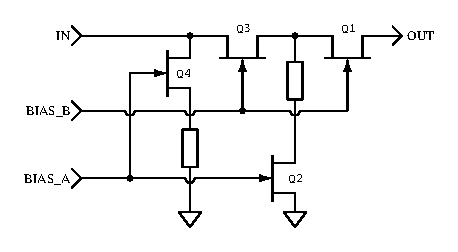
\includegraphics{too/gaassw}
\caption{GaAs switch circuit}
\label{fig:gaassw}
\end{figure}

Figure~\ref{fig:gaassw} shows the internal circuit of the
switch~\cite{maswss0162}.  It is a simple circuit built from four gallium
arsenide (GaAs) FETs \footnote{The type of FET used is a relatively uncommon
    variant called a \emph{MESFET}, or MEtal-Semiconductor Field Effect
Transistor. This is a variant on the well known JFET, using a Schottky junction
instead of a PN junction. While uncommon in general, it is used often in GaAs
circuits due to the relative ease of constructing GaAs MESFETs.}.  These are
depletion-mode devices, so they are switched \emph{on} by applying zero volts
to the gate, and turned \emph{off} by applying a negative voltage, around
\Neg 5~V.  Switching on transistors \refdes{Q1} and \refdes{Q3} allows the
signal to pass through from the input to the output. Switching on transistors
\refdes{Q2} and \refdes{Q4} disconnects the input from the output, but also
\emph{terminates} the input (applies a $50\;\Omega$ resistance between the
input and ground). This is important to make sure that a disconnected input
does not cause signal reflections.

\begin{figure}[H]
\centering
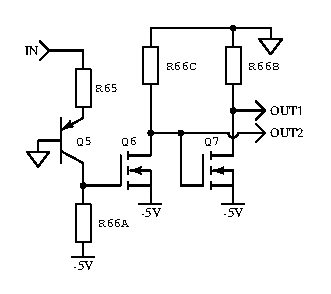
\includegraphics{too/gaasctl}
\caption{GaAs control circuit}
\label{fig:gaasctl}
\end{figure}

Figure~\ref{fig:gaasctl} is the control circuit for figure~\ref{fig:gaassw}.
When 0~V (a logic \emph{low}) is applied to the input from the
microcontroller, no current flows through \refdes{R65} or \refdes{R66A}.
This applies \Neg 5~V to \refdes{Q6}. Because \refdes{Q6}'s source is
connected to the \Neg 5~V rail instead of ground, the voltage between gate
and source ($V_{GS}$) is zero, and \refdes{Q6} is switched off.
This provides 0~V to one input of the GaAs switches. \refdes{Q7} acts
as an inverter, providing \Neg 5~V to the other GaAs switch input. The
dual switches have their inputs connected opposite each other, so this
switches one of them \emph{on} and the other \emph{off}.

When 3.3~V (a logic \emph{high}) is applied to the input from the
microcontroller, about 1.6~mA flows through \refdes{R65}. This
saturates \refdes{Q5}, applying about 0.7~V to \refdes{Q6}. As above,
$V_{GS}$ is the difference between this and the \Neg 5~V rail, or
5.7~V. \refdes{Q6} now switches on, and the two signals to the GaAs
switches swap places. This swaps the two switches, turning on the one that was
off, and turning off the one that was on.


\subsubsection{Buffer and Filter}
\schematicpage{9}{Buffer\_Filter}

\begin{figure}[H]
\centering
\missingfigure[figwidth=3in]{buffer}
\caption{Input buffer circuit}
\label{fig:buffer}
\end{figure}

Figure~\ref{fig:buffer} is the input signal buffer. \refdes{Q9} is a simple
emitter-follower (common collector) amplifier, providing isolation
between the input and further circuitry. \refdes{Q10} and \refdes{Q8} form
a current source to power it, in a feedback configuration providing
approximately $0.65\;\mr{V} / 30\;\Omega \approx 22\;\mr{mA}$.

The configuration of \refdes{R76} and \refdes{R77} sums together
the input signal and the phase reference signal, and this continues to the
input filter. \refdes{R75} combines with \refdes{R76} to properly
terminate the 50~\Ohm{} phase reference signal.

To lower the effect of external interference on the signals, a filter restricts
signals above the instrument's maximum operating frequency from continuing
past this point.

\subsubsection{Logarithmic Detector}
\schematicpage{10}{Detector}

Signals at this point can have a very wide variety of amplitudes, as high as \Pos 10~dBm
(1~V peak) and as low as \Neg 60~dBm (224~\uV{} peak) or even lower, and over a wide
frequency range. Measuring this requires a \emph{logarithmic detector}. This is a
circuit that responds to the logarithm of the signal, rather than the signal itself,
generating a voltage proportional to the \emph{decibel} amplitude of the signal. More
exactly, the output voltage of the detector is equal to:

\begin{equation*}
    V_\mathrm{out} = (24\;\mr{mV/dB})((20\;\mr{dB})\log_{10}(V_\mathrm{in}) + 108\;\mr{dB})
\end{equation*}
